\documentclass{article}
\usepackage{tikz}
\usepackage{amsmath}
\usepackage{anyfontsize}

\begin{document}

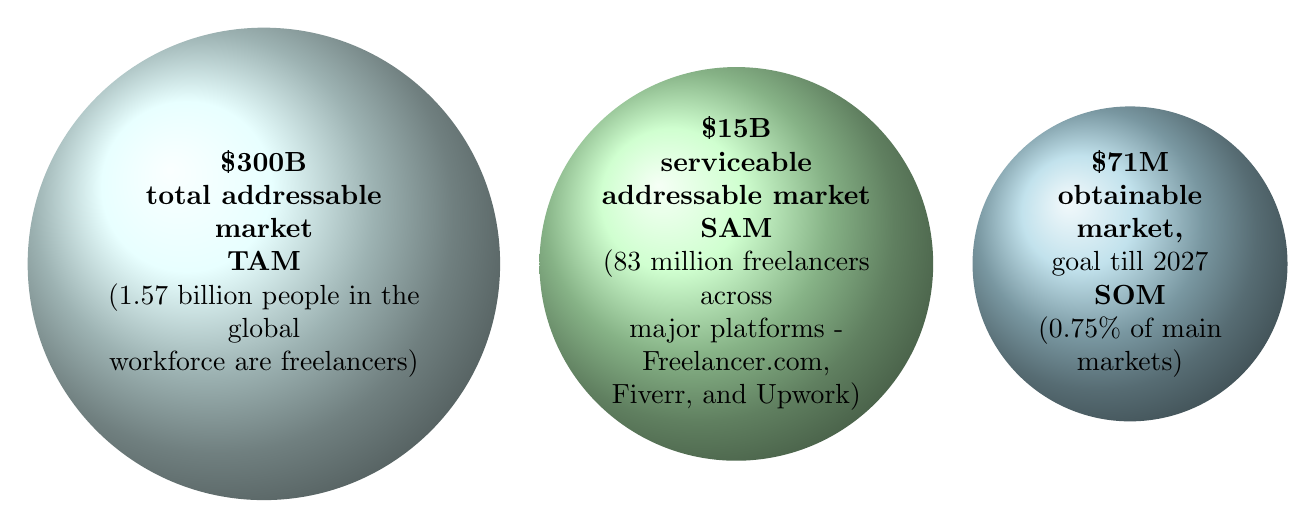
\begin{tikzpicture}

    % Colors for the circles
    \definecolor{lightblue}{RGB}{173,216,230}
    \definecolor{lightgreen}{RGB}{192,255,192}
    \definecolor{lightcyan}{RGB}{224,255,255}
    
    % TAM Circle
    \shade[ball color=lightcyan] (-6,0) circle (3cm);
    \node at (-6,0) {\parbox{4cm}{
        \centering
        \textbf{\$300B}\\
        \textbf{total addressable market}\\
        \textbf{TAM}\\
        (1.57 billion people in the global\\
        workforce are freelancers)
    }};

    % SAM Circle
    \shade[ball color=lightgreen] (0,0) circle (2.5cm);
    \node at (0,0) {\parbox{4cm}{
        \centering
        \textbf{\$15B}\\
        \textbf{serviceable addressable market}\\
        \textbf{SAM}\\
        (83 million freelancers across\\
        major platforms - Freelancer.com,\\
        Fiverr, and Upwork)
    }};

    % SOM Circle
    \shade[ball color=lightblue] (5,0) circle (2cm);
    \node at (5,0) {\parbox{3cm}{
        \centering
        \textbf{\$71M}\\
        \textbf{obtainable market,}\\
        goal till 2027\\
        \textbf{SOM}\\
        (0.75\% of main markets)
    }};
    
\end{tikzpicture}

\end{document}
